\chapter{Resultados e Validação} \label{ch:results}

\alert{Lembrar que é necessário validar as coisas}

Este capítulo dedica-se à apresentação de resultados e validação numérica 

\alert{Terminar de dizer por que este capítulo existe}

\section{Lançamento Oblíquo}

O lançamento oblíquo é um dos problemas clássicos de física básica. Considera-se uma partícula de massa sujeita unicamente à ação de um campo gravitacional constante cuja aceleração da gravidade é \(\gravity\). Nessas condições, as equações de movimento para a partícula se tornam, simplesmente,
\begin{gather}
	\acceleration = \gravity, \label{eq:free_fall_translation}\\
	\angularAcceleration = \nullVector \label{eq:free_fall_rotation}.
\end{gather}

O instante inicial da simulação é definido como \(\initial{t}=0\), e o instante final é um valor arbitrário \(\final{t}\). A posição, a velocidade e a velocidade angular da partícula no instante inicial assumem, respectivamente, os valores \(\initial{\position}\), \(\initial{\velocity}\) e \(\initial{\angularVelocity}\). As equações \eqref{eq:free_fall_translation} e \eqref{eq:free_fall_translation} podem ser resolvidas por integração simples:
\begin{gather*}
	\acceleration\pqty{t} = \gravity, \\
	\velocity\pqty{t} = \initial{\velocity} + \int_{0}^{t} \acceleration\pqty{\tau} \dd{\tau} = \initial{\velocity} + \gravity\cdot t, \\
	\position\pqty{t} = \initial{\position} + \int_{0}^{t} \velocity\pqty{\tau} \dd{\tau} = \initial{\position} + \initial{\velocity}\cdot t + \gravity\cdot \dfrac{t^2}{2}, \\
	\angularVelocity\pqty{t} = \initial{\angularVelocity} + \int_{0}^{t} \nullVector \dd{\tau} = \initial{\angularVelocity}.
\end{gather*}

Por simplicidade, considera-se que o movimento ocorra apenas no plano \(\xAxis\yAxis\), que a gravidade atue no sentido negativo do eixo \(\yAxis\), isto é, \(\gravity = \gravityScalar\cdot\yUnit\) com \(\gravityScalar<0\), e que a partícula não possua rotação, como representado na figura \ref{fig:free_fall}.

\begin{figure}[h]
	\caption{O problema do lançamento oblíquo}
	% \vspace{-0.5cm}
	\begin{center}
		\alert{Colocar imagem representando o problema do lançamento oblíquo}
		% 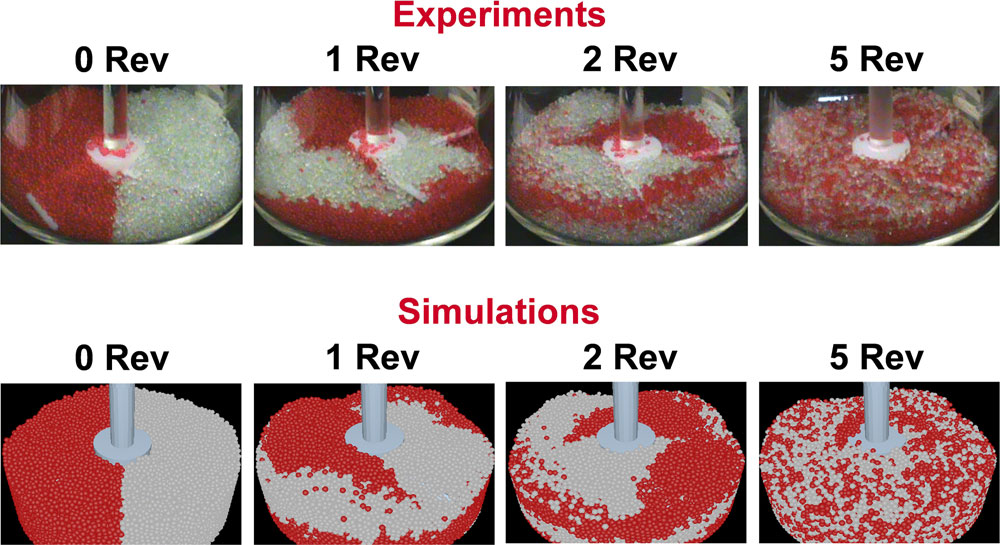
\includegraphics[width=0.65\textwidth]{images/drug_production.png}
	\end{center}
	% {\centerline{\includegraphics[scale=#2]{#1}}}
	% \vspace{-0.2cm}
	\label{fig:free_fall}
	\legend{Fonte: \alert{Citar fonte}.}
	% \vspace{-1cm}
\end{figure}

Com isso, escrevendo \(\position = \explicitVectorCoordinates{\positionScalar}\), \(\velocity = \explicitVectorCoordinates{\velocityScalar}\) e \(\acceleration = \explicitVectorCoordinates{\accelerationScalar}\), é obtida a solução como apresentada na tabela \ref{table:free_fall_solution}.

\alert{Consertar a seguinte tabela:}

\begin{table}[h]
	\caption{Solução do problema do lançamento oblíquo}
	\label{table:free_fall_solution}

	\begin{equation*}
		% \arraycolsep=1.4pt
		\def\arraystretch{1.5}
		\begin{array}{lccc}
	\hline
		& \text{Direção } \xAxis & \text{Direção } \yAxis & \text{Direção } \zAxis \\
		\text{Posição} & \xComponent{\position} = \initial{\xComponent{\position}} + \alert{Continuar e corrigir notação anterior} & & \\
	\hline	
		\end{array}
	\end{equation*}
	\legend{Fonte: do Autor}
\end{table}

Embora seja um problema conceitualmente simples e de fácil resolução, o problema do lançamento oblíquo permite a validação numérica da implementação do algoritmo de Gear.

\alert{Na verdade, valida apenas a parte de previsão e, parcialmente, o corretor. Isso porque o erro de aceleração é zero...}

\alert{Mostrar o quanto o erro evolui com o aumento do tempo final de simulação}

\alert{Seria interessante de se colocar uma enumeração ilustrando todos os aspectos do programa validados}

\subsection{Exemplo de Solução} \alert{Que título horrível!}



\subsection{Influência da Ordem de Extrapolação}

\subsection{Influência do Passo de Tempo}